\documentclass[10pt,a4]{article}
% \usepackage{draftwatermark}
\usepackage{color}\usepackage{pdfpages}
\usepackage{background}
\usepackage{color}   %May be necessary if you want to color links
\usepackage{hyperref}
\hypersetup{
    colorlinks=true, %set true if you want colored links
    linktoc=all,     %set to all if you want both sections and subsections linked
    linkcolor=blue,  %choose some color if you want links to stand out
}
\textwidth 170 mm
\oddsidemargin -8 mm
\evensidemargin -8 mm
%\SetWatermarkScale{3.0}
\SetBgColor{red}
\SetBgOpacity{0.1}
\SetBgScale{10}
%\SetBgContents{\hspace{9mm}DRAFT \hspace{0mm}\vspace{2mm} \includegraphics[width=5mm]{Alfresco_logo_CMYK_white}} 

\newcommand{\fasterold}{{\bf We do it FASTER:\ }}
\newenvironment{faster}{{\bf {\color{red}We do it FASTER:}} \em}{\par\normalfont}% \slshape\itshape

\begin{document}
\begin{center}
{\huge A faster installation of Alfresco}

\vspace{5mm}

\Large{on IBM Websphere Application Server WAS7}

\vspace{25mm}

{\bf Alex Madon}

\vspace{5mm}

Alfresco Support

\vspace{5mm}

\today

\vspace{15mm}
{\huge To be reviewed}

\end{center}
\vspace{5mm}

\newpage

\tableofcontents

\newpage

\section{Introduction}
\subsection{Motivation}
The official documentation of Alfresco \cite{officialdoc} presents a procedure to install Alfresco on Websphere. It does not include how to install Websphere itself. This is understandable, because this is a documentation about Alfresco and not about IBM Websphere.
The steps to install Alfresco itself are accurately described; However, they are time consuming.

In Alfresco support team, we need to be able to create test setup to reproduce issues. This document includes a full installation process, i.e that includes Websphere installation. Also, in a support team, we have to do install very quickly. In fact because each customer's environment is different, we have to create very quickly an stack. 

In this document, we present how to install Websphere, in the fastest way possible. This includes the setup of the JDBC configuration to any database. We present here as an example a setup with a postgresql back-end, but adapting the instructions for mysql, or oracle would be as easy as changing a JAR file name. Similarly, changing the version of alfresco would be as easy as changing few characters in the input files of the installer automata.

In this document, we also present an alternative way of installing alfresco within Websphere. This installing is automated. All the instructions are given to have a completely automated installation process without any human interaction other than passing configuration parameters to a command line program or in a installer configuration file.


\subsection{Target audience}
This document presents methods to create disposable tests environments. As such it would be useful to engineers in Support, QA and Development teams. With Little work, it could also be adapted to Production teams.

\subsection{Disclaimer}
This method of installation is for testing only (Support, QA), not for Production. For production, security improvements needs to be considered in particular protect the WAS admin page with passwords and maybe remove some of the unused Sample applications.


\section{For busy people}
As mentioned in the introduction, the whole installation process could be reduced to the call of one command; We present here the fastest way to create a Websphere environment, that is all the commands that need to be run. Those steps do not involve any access to the Websphere web console \url{http://localhost:9060/ibm/console/}. Then, later on in the document, we go back to each of the steps and detail what we are doing and why.


In the below  \textasciitilde\  refers to the home directory of the user who install WAS. We use \textasciitilde\  but in cases we need absolute paths we use /home/madon. The commands listed below are for the installation of alfresco on Linux (Debian) with postgresql.


\begin{enumerate}
\item Install some compatibility packages:
\begin{verbatim}
sudo apt-get install ia32-libs
\end{verbatim}
\item Get the WAS software, i.e. the file 
\begin{verbatim}
was.cd.70011.trial.base.opt.linux.ia32.tar.gz
\end{verbatim}
from:
\url{https://www14.software.ibm.com/webapp/iwm/web/pick.do?S_SRCID=was60&source=was60&S_CMP=web_dw_rt_swd&S_TACT=109J84IW&lang=en_US}

and save it into e.g. {\tt \textasciitilde/websphere}
\item uncompress it:
\begin{verbatim}
cd ~/websphere
tar -xzvf was.cd.70011.trial.base.opt.linux.ia32.tar.gz
cd WAS
\end{verbatim}
create a file file alfresco\_ports.props:
\begin{verbatim}
WC_defaulthost=8080
\end{verbatim}
\item Create a file {\tt responsefile.base.txt} in the directory {\tt \textasciitilde/websphere/WAS} which contains:
\begin{verbatim}
# ================================================================
# Alfresco Websphere response file; To run:
# java -jar setup.jar -silent -options responsefile.base.txt 
# ================================================================
-OPT installLocation=/home/madon/IBM/WebSphere/AppServer
-OPT installType=installNew
-OPT feature=samplesSelected
-OPT allowNonRootSilentInstall=true
-OPT silentInstallLicenseAcceptance=true
-OPT traceLevel=DEBUG
-OPT disableOSPrereqChecking=true
-OPT PROF_enableAdminSecurity=false
-OPT PROF_isDefault=true
-OPT PROF_appServerProfileName=AppSrv01
-OPT PROF_portsFile=alfresco_ports.props
\end{verbatim}
\item Create a file {\tt alfresco\_ports.props} in the directory {\tt \textasciitilde/websphere/WAS} which contains:
\begin{verbatim}
WC_defaulthost=8080
\end{verbatim}

\item Install Websphere
\begin{verbatim}
java -jar setup.jar -silent -options responsefile.base.txt 
\end{verbatim}
optionally watching the logs:
\begin{verbatim}
tail -f ~/waslogs/trace.txt
\end{verbatim}

Note: if install hangs on importConfigArchive

then check that bin sh does not point to bin dash
If it does, then link it to  bin bash

\begin{verbatim}
cd /bin
ls -lh sh
rm sh
ln -s  bash sh
ls -lh sh
\end{verbatim}


\item Create a directory for the alfresco data:
\begin{verbatim}
mkdir ~/was_alf_data
\end{verbatim}



\item create a Postgresql database:

\begin{verbatim}
# dropdb -Ualfresco alfresco415was
createdb -Ualfresco alfresco415was
\end{verbatim}


\item Create a keystore folder and generate a keystore:

\begin{verbatim}
# Create a keystore folder
mkdir ~/waskeystore/
cd  ~/waskeystore/
# Generate the keystore
~/IBM/WebSphere/AppServer/java/bin/keytool -genseckey -alias metadata \
-keypass mypass2 -storepass mypass1 -keystore keystore \
-storetype JCEKS -keyalg DESede
\end{verbatim}

\item Create a file {\tt keystore-passwords.properties} in the keystore folder that contains the following lines:

\begin{verbatim}
aliases=metadata
# The password protecting the keystore entries
keystore.password=mypass1
# The password protecting the alias: metadata
metadata.keyData=
metadata.algorithm=DESede
metadata.password=mypass2
\end{verbatim}
\item Install myfaces:
\begin{verbatim}
cd ~/IBM/WebSphere/AppServer
cp ~/tmp/myfaces1_1-websphere-shared-lib-4.1.4.zip .
unzip myfaces1_1-websphere-shared-lib-4.1.4.zip 
\end{verbatim}

\item launch and configure WAS:
\begin{verbatim}
cd ~/IBM/WebSphere/AppServer/bin
./startServer.sh server1
./wsadmin.sh -lang jython 

server = AdminConfig.getid("/Server:server1/")

# increase the Max Heap:
jvmid = AdminConfig.list("JavaVirtualMachine", server)
AdminConfig.show(jvmid).splitlines()
attrs = [["maximumHeapSize", 2048]]
AdminConfig.modify(jvmid, attrs)

# workaround IE bugs, see MNT-3525
services=AdminConfig.list("TransportChannelService",server)
channels=AdminConfig.list("HTTPInboundChannel",services)
opts=[]
opts.append(["validationExpression", ""])
opts.append(["name", "CookiesConfigureNoCache"])
opts.append(["description", "workaround IE6,7,8 bug see MNT-3525"])
opts.append(["value", "false"])
opts.append(["required", "false"])
for http in channels.split("\n"):
    hname=AdminConfig.showAttribute(http, "name")
    if  hname=="HTTP_2":
        print ("Setting CookiesConfigureNoCache to false for", http)
        AdminConfig.create("Property",http,opts)

# saving config
AdminConfig.save()
\end{verbatim}

Note: you can write all the jythin commands to a file called script1.py and then execute it with:


\begin{verbatim}
wsadmin.sh -lang jython -f  script1.p
\end{verbatim}


\item Get the Alfresco EAR ZIP file for the support page, and save it into e.g  {\tt \textasciitilde/tmp}
\begin{verbatim}
mkdir ~/tmp ~/was_alf_data
cd ~/tmp
unzip alfresco-enterprise-ear-4.1.4.zip
cp ~/alfresco_soft/postgresql-9.0-802.jdbc4.jar ~/IBM/WebSphere/AppServer/lib

cd ~/IBM/WebSphere/AppServer/lib
cp ~/tmp/web-server/classpath/alfresco-global.properties.sample alfresco-global.properties
# append properties to your alfresco-global.properties file
echo "
mbean.server.locateExistingServerIfPossible=false
dir.root=/home/madon/was_alf_data
dir.keystore=/home/madon/waskeystore/

db.driver=org.postgresql.Driver
db.url=jdbc:postgresql://localhost/alfresco415was
db.username=alfresco
db.password=alfresco

" >> alfresco-global.properties
\end{verbatim}


\item Deploy Alfresco:
\begin{verbatim}
cd ~/IBM/WebSphere/AppServer/bin
./wsadmin.sh -lang jython 
# deploy Alfresco
earpath="/home/madon/tmp/alfresco-enterprise-4.1.4.ear"
mapref=[]
mapref.append("Alfresco Web Client")
mapref.append("")
mapref.append("alfresco.war,WEB-INF/web.xml")
mapref.append("jdbc/dataSource")
mapref.append("javax.sql.DataSource")
mapref.append("jdbc/dummy")
mapref.append("")
mapref.append("")
mapweb=[]
mapweb.append(["Alfresco Web Client", "alfresco.war,WEB-INF/web.xml", "default_host"])
mapweb.append(["Alfresco Project Slingshot", "share.war,WEB-INF/web.xml", "default_host"])
AdminApp.install(earpath, ["-server", "server1", "-MapResRefToEJB", [mapref],"-MapWebModToVH",mapweb])
AdminConfig.save()
\end{verbatim}

\item Restart the server:

\begin{verbatim}
cd ~/IBM/WebSphere/AppServer/bin
./stopServer.sh server1
./startServer.sh server1
\end{verbatim}
Optionally monitor the boot logs:
\begin{verbatim}
tail -f ~/IBM/WebSphere/AppServer/profiles/AppSrv01/logs/server1/SystemOut.log
\end{verbatim}
\item optionally, turn off the flash uploader (see \cite{MNT-9757}) as per the official doc.
\end{enumerate}

\section{Comparison with official documentation}
The next page shows a screen shot of the current 4.1 documentation presenting the installation steps to follow to install Alfresco on Websphere. Fonts have been scaled down to fit the page.
% \includegraphics[width=90mm]{official2}
\includepdf[pages={1}]{official6}

\section{Websphere response files}
\subsection{Silent (non interactive) installation}
IBM allows installation of many of its software using so-called ``response files''.
An installation without options passed at the command line, e.g:
\begin{verbatim}
java -jar setup.jar
\end{verbatim}
will launch a graphical interface and several screens will be presented. We shows the first five screens in picture \ref{sc1}.% to \ref{sc5}.
This is useful and interesting the first time you install WAS but becomes annoying when you have to install and re-install the product many times. 



However, the response to each screen and in fact the whole configuration can be defined in files called ``response files''.

\begin{faster}
We use ``response files'' to have a fully automated WAS installation.
\end{faster}


The syntax to call a response file is:

\begin{verbatim}
java -jar setup.jar -silent -options responsefile.base.txt 
\end{verbatim}

The response file we use in our example installation is:

\begin{verbatim}
# ================================================================
# Alfresco Websphere response file; To run:
# java -jar setup.jar -silent -options responsefile.base.txt 
# ================================================================
-OPT installLocation=/home/madon/IBM/WebSphere/AppServer
-OPT installType=installNew
-OPT feature=samplesSelected
-OPT allowNonRootSilentInstall=true
-OPT silentInstallLicenseAcceptance=true
-OPT traceLevel=DEBUG
-OPT disableOSPrereqChecking=true
-OPT PROF_enableAdminSecurity=false
-OPT PROF_isDefault=true
-OPT PROF_appServerProfileName=AppSrv01
-OPT PROF_portsFile=alfresco_ports.props
\end{verbatim}

In a QA or Support environment, you probably will have to change only the path, i.e. the {\tt installLocation} option. In production you will have to change the security parameters in particular {\tt PROF\_enableAdminSecurity} and probably also the {\tt feature} option as it installs test applications.

\begin{figure}[htb]
\begin{center}
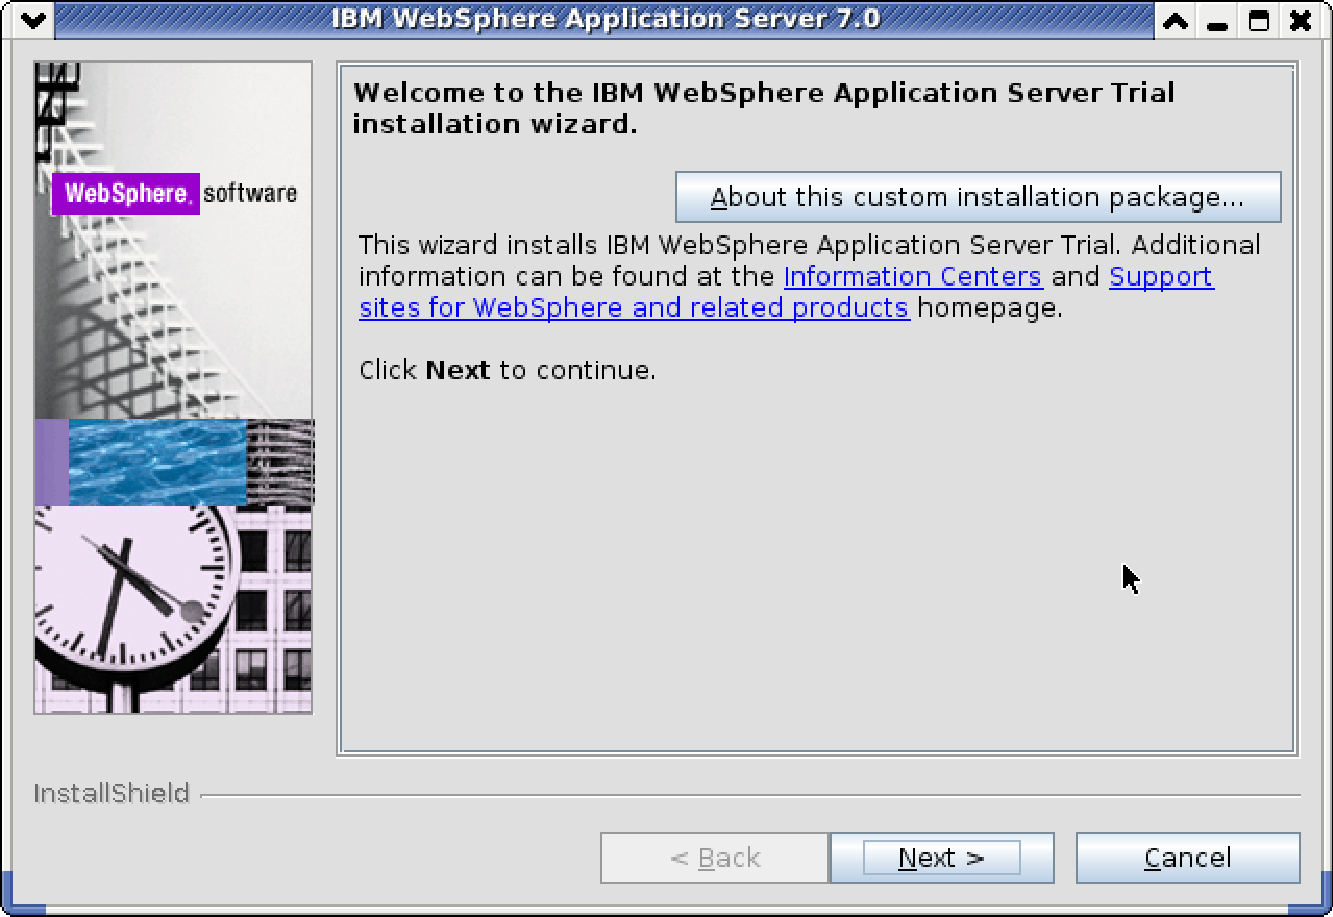
\includegraphics[width=90mm]{ws01}
\caption{WAS7 Graphical installation, screen 1.}
\label{sc1}
\end{center}
\end{figure}

%\begin{figure}[htb]
%\begin{center}
%\includegraphics[width=90mm]{ws02}
%\caption{WAS7 Graphical installation, screen 2.}
%\label{sc2}
%\end{center}
%\end{figure}

%\begin{figure}[htb]
%\begin{center}
%\includegraphics[width=90mm]{ws03}
%\caption{WAS7 Graphical installation, screen 3.}
%\label{sc3}
%\end{center}
%\end{figure}

%\begin{figure}[htb]
%\begin{center}
%\includegraphics[width=90mm]{ws04}
%\caption{WAS7 Graphical installation, screen 4.}
%\label{sc4}
%\end{center}
%\end{figure}

%\begin{figure}[htb]
%\begin{center}
%\includegraphics[width=90mm]{ws05}
%\caption{WAS7 Graphical installation, screen 5.}
%\label{sc5}
%\end{center}
%\end{figure}


\subsection{Changing the port to 8080}
In the official documentation we have a very long paragraph about changing the ports in the {\tt share-config-custom.xml} file. Changing Share connectivity to Alfresco is complex, difficult to explain (see the number of documentation lines dedicated to that change), difficult to do (error prone) and difficult to understand especially to new hires.

\begin{faster}
In our case we just modify the port configuration of Websphere to match Share default configuration which assumes Alfresco runs on localhost on port 8080. This is much faster that changing Share configuration to connect to Websphere default HTTP port 9080.
\end{faster}

This change in Websphere configuration is done in two very easy steps:
\begin{enumerate}
\item add one line to the response file:
\begin{verbatim}
-OPT PROF_portsFile=alfresco_ports.props
\end{verbatim}
\item and then create a one line file called {\tt alfresco\_ports.props}
\begin{verbatim}
WC_defaulthost=8080
\end{verbatim}
\end{enumerate}

\section{Automating changes to the application}
The official documentation details how to modify the default server settings using the Websphere web console located at \url{http://localhost:9060/ibm/console/}. Documenting operations in a web interface is complex and the properties are located in deep trees. Moreover, the URLs to use as a shortcut to get directly to the HTML form were a parameter can be modified is long and barely readable by humans. e.g. to go to the custom property interface to add the CookiesConfigureNoCache parameter (see step 8c of the official documentation)

{\bf
Application servers \textgreater\ server1 \textgreater\ Web container \textgreater\ Web container transport chains \textgreater\ HttpQueueInboundDefault \textgreater\ HTTP inbound channel (HTTP\_2) \textgreater\ Custom properties
}

the URL is

\begin{verbatim}
http://localhost:9060/ibm/console/com.ibm.ws.console.channelfw.forwardCmd.do?
forwardName=Property.content.main&sfname=properties&lastPage=HTTPInboundChannel.config.view
&resourceUri=server.xml&parentRefId=HTTPInboundChannel_1183122130079
&contextId=cells%3AmadonaNode01Cell%3Anodes%3AmadonaNode01%3Aservers%3Aserver1&perspective=tab.configuration
\end{verbatim}


\begin{figure}[htb]
\begin{center}
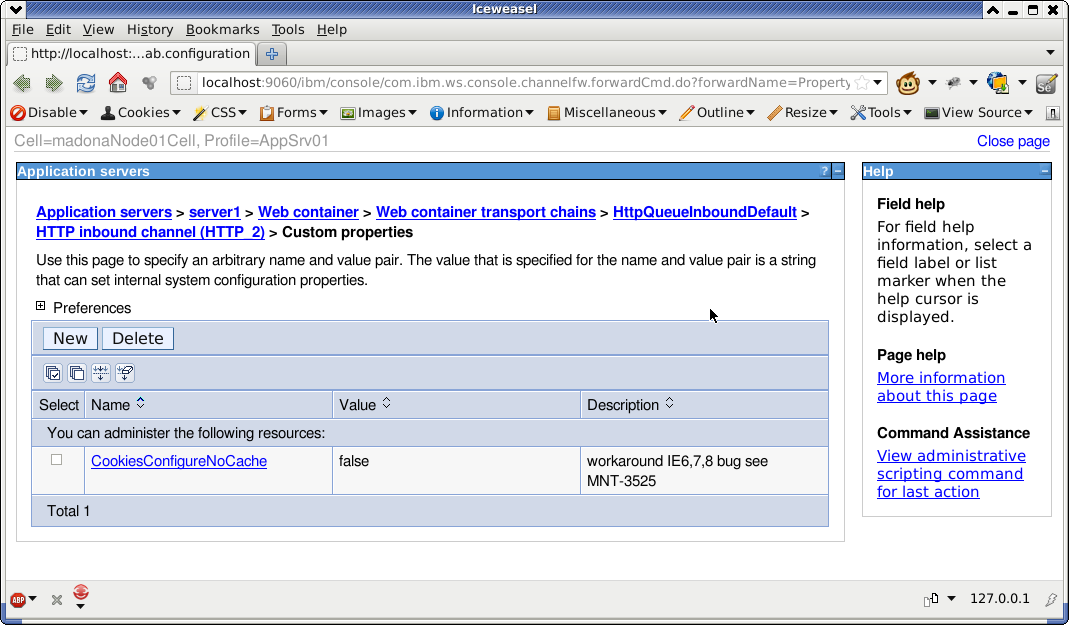
\includegraphics[width=130mm]{cookie}
\caption{Custom properties interface}
\label{sc1}
\end{center}
\end{figure}

\begin{faster}
We use the {\tt wsadmin} program.
\end{faster}

IBM WAS official documentation documents\cite{wsadminjython} how to automate using scripting changes to a server.
This is done using the {\tt wsadmin} program. As mentioned by the IBM documentation, there are two programming languages available: JACL and Jython. As Jacl is being deprecated\cite{wsadminjython} since WAS 6.1, we show in this document the Jython syntax. Jython \cite{jython} is an implementation of the Python programming language written in Java. Whereas the official Python distribution is written in C, Jython allows naturally the use of the Java code and classes embedded in IBM Websphere.

The {\tt wsadmin} program normally resides in the same directory than the {\tt startServer.sh} and {\tt stopServer.sh}, that is in our example in {\tt \textasciitilde\ /IBM/WebSphere/AppServer/bin}

\begin{verbatim}
madon@madona:~/IBM/WebSphere/AppServer/bin$ ./wsadmin.sh -h
....
-c <command>
....
-f <script_file_name>
....
-lang  language
....
\end{verbatim}
To using the Jython syntax you will have to use the {\tt -lang jython} option.
If you do not use the {\tt -c} or {\tt -f} options then an interactive session will be launched where you can enter one by on each of the commands.

Using the  {\tt -c}  allows you to execute Jython commands passed as a command line argument.
Using the  {\tt -f}  allows you to execute a full Jython script.

\subsection{Setting JVM options using wsadmin}

The increase of the Heap mentioned at step 8)b) of the official documentation can be translation into the below Jython script:

\begin{verbatim}
server = AdminConfig.getid("/Server:server1/")

# increase the Max Heap:
jvmid = AdminConfig.list("JavaVirtualMachine", server)
AdminConfig.show(jvmid).splitlines()
attrs = [["maximumHeapSize", 2048]]
AdminConfig.modify(jvmid, attrs)
AdminConfig.save()
\end{verbatim}


\subsection{Setting CookiesConfigureNoCache to False using wsadmin}

The creation of the custom variable {\tt CookiesConfigureNoCache} at step 8)c) of the official documentation can be translation into the below Jython script:
\begin{verbatim}
server = AdminConfig.getid("/Server:server1/")
# workaround IE bugs, see MNT-3525
services=AdminConfig.list("TransportChannelService",server)
channels=AdminConfig.list("HTTPInboundChannel",services)
opts=[]
opts.append(["validationExpression", ""])
opts.append(["name", "CookiesConfigureNoCache"])
opts.append(["description", "workaround IE6,7,8 bug see MNT-3525"])
opts.append(["value", "false"])
opts.append(["required", "false"])
for http in channels.split("\n"):
    hname=AdminConfig.showAttribute(http, 'name')
    if  hname=="HTTP_2":
        print ("Setting CookiesConfigureNoCache to false for", http)
        AdminConfig.create("Property",http,opts)

# saving config
AdminConfig.save()
\end{verbatim}

\subsection{Creating the Alfresco-style datasource}
As mentioned in the old wiki\cite{wikiwas} there are two ways to create a connection pool to a database in Websphere: the Websphere way and the Alfresco way. The official documentation only describes the Alfresco way and this is the only method officially supported.
The creation of an Alfresco-style connection pool and the deployment of the Alfresco and Share applications can be achieved using the following Jython script for wsadmin:

\begin{verbatim}
# deploy Alfresco
earpath="/home/madon/tmp/alfresco-enterprise-4.1.4.ear"
mapref=[]
mapref.append("Alfresco Web Client")
mapref.append("")
mapref.append("alfresco.war,WEB-INF/web.xml")
mapref.append("jdbc/dataSource")
mapref.append("javax.sql.DataSource")
mapref.append("jdbc/dummy")
mapref.append("")
mapref.append("")
mapweb=[]
mapweb.append(["Alfresco Web Client", "alfresco.war,WEB-INF/web.xml", "default_host"])
mapweb.append(["Alfresco Project Slingshot", "share.war,WEB-INF/web.xml", "default_host"])
AdminApp.install(earpath, ["-server", "server1", "-MapResRefToEJB", [mapref],"-MapWebModToVH",mapweb])
AdminConfig.save()
\end{verbatim}

\subsection{Keystores}
The creation of a customer keystore is not a requirement as per the official documentation. However I raised a Jira\cite{MNT-9737} as it was needed for me. The Jira is still open.

\subsection{Alfresco global properties files}
The {\tt alfresco-global.properties} file also needs to be modified. This can easily b scripted using any language and I won't detail that step here.

\section{Tip to map UI changes to wsadmin changes}
Finally I would like to note that there is a nice command that you can call from {\tt wsadmin} which allows you to dump your current Websphere configuration. This could be use to reverse engineer the documentation, i.e., you dump your configuration before doing the change in the web UI, then you do the change in the Web UI, then you do a new dump of the configuration.
To see what configuration variable are affected by the web UI change, you just have to a do a ``diff'' between the two versions of the configuration dumps. Those files are typically very large, but the ``diff'' command will show you was exactly the change was; and the change is typically only few lines long. The format of the file is not a set of Jython commands, but could relatively easily mapped to Jython commands.
The command to generate the dump is ``AdminTask.extractConfigProperties''; Example:
\begin{verbatim}
cd ~/IBM/WebSphere/AppServer/bin
./wsadmin.sh -lang jython 
AdminTask.extractConfigProperties('-propertiesFileName props1.props')
\end{verbatim}
There is also a command to re-inject a complete properties file: {\tt applyConfigProperties} see \cite{moreadmin} for more details.


\section{Conclusion}
In this document we have presented a way to semi-automate or fully automate the setup of Websphere environments for testing or doing QA on Alfresco. This could help improving the productivity of the Support, QA or even Dev teams allowing those teams to concentrate of the actual issue to be investigated/tested.


\begin{thebibliography}{9}

\bibitem{officialdoc}
\url{http://docs.alfresco.com/4.1/topic/com.alfresco.enterprise.doc/tasks/alf-websphere-install.html}

\bibitem{MNT-9737}
\url{https://issues.alfresco.com/jira/browse/MNT-9737} 

Document need of keystore generation when installing on IBM Websphere Application Server (WAS)

\bibitem{MNT-9757}
\url{https://issues.alfresco.com/jira/browse/MNT-9757} 

On Websphere Flash uploader fails with "HTTP/1.1 401 No USER\_ID found in session and requested endpoint requires authentication."

\bibitem{wsadminjython}

\url{http://pic.dhe.ibm.com/infocenter/rsahelp/v8/index.jsp?topic=\%2Fcom.ibm.jythontools.doc\%2Ftopics\%2Fcautoscript.html}


\bibitem{jython}
\url{http://en.wikipedia.org/wiki/Jython}

\bibitem{wikiwas}
\url{http://wiki.alfresco.com/wiki/Installing_on_WebSphere}

\bibitem{moreadmin}

\url{http://pic.dhe.ibm.com/infocenter/wasinfo/v8r0/index.jsp?topic=\%2Fcom.ibm.websphere.express.doc\%2Finfo\%2Fexp\%2Fae\%2Frxml_7propbasedconfig.html}

 \end{thebibliography}


\end{document}
